\mode*

Pharmakodynamik beschreibt die Beziehung zwischen der (Wirkort-) Konzentrtion und der Wirkung. \\
Wenn sich ein Agonist an den Rezeptor bindet, entfaltet er eine Wirkung. Wenn sich der 
Antagonist an den Receptor bindet, \enquote{passiert nichts}. Falls
eine gewisse (partielle) Wirkung entfaltet wird spricht man von
einem partiellen Agonisten. Auch bei sehr hohen Konzentrationen kann mit einem partiellen Agonisten nicht dieseselbe Wirkung erzielt werden wie mit dem vollen Agonisten. Diese sind gleichszeitig auch partielle Antagonisten wegen Kompetition am Rezeptor.\\
Die Potenz beschreibt wie wirksam das Medikament im Verh�ltnis zur Konzentration (Menge) ist. Die Konzentration die 50\% der maximalen Wirkung ($EC_{50}$) erreicht, ist ein Mass f�r die Potenz.
Die Potenz eines Medikamentes ist eher nebens�chlich, solange das Medikament mengenm�ssig vern�nftig zugef�hrt werden kann.



\frame{
\frametitle{Pharmakodynamik - Begriffe}
\begin{block}{}
    \begin{itemize}
        \item Agonist, Antagonist, part. Antagonist, inverser
        Agonist
        \item Potenz
        \item (max.) Wirksamkeit (Efficacy)
        \item Steigung
    \end{itemize}
\end{block}
\note<1>{.}
}

Die Steigung der Konzentrations - Wirkungsbeziehung muss ebenfalls beachtet werden. Wenn die Steigung flach ist,
braucht es einen gr�sseren Konzentrationsabfall f�r einen bestimmten Wirkungsabfall.
 



\frame{
\frametitle{Potenz, Wirksamkeit (Efficacy)}
\begin{block}{}
\mode<presentation>{
    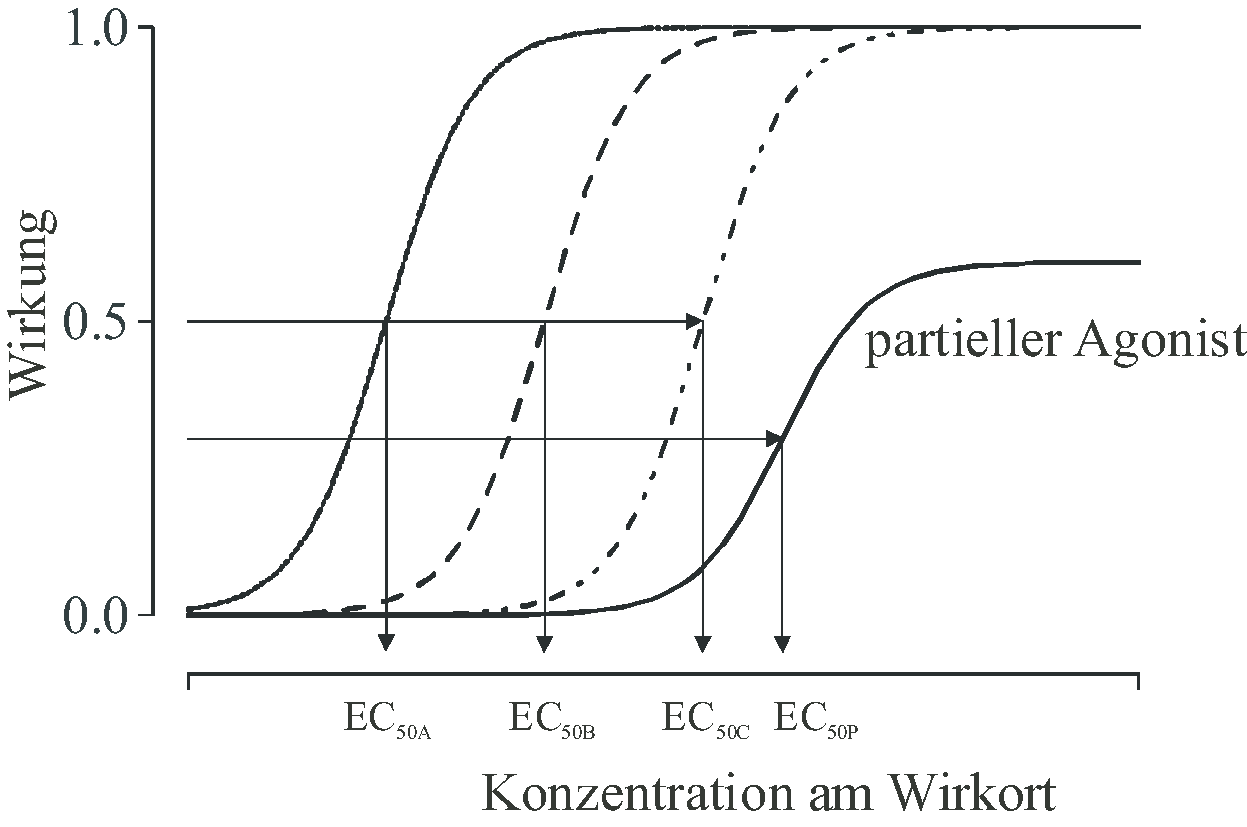
\includegraphics[clip=true,width=0.8\textwidth]{./pd2.pdf}
}
\mode<article>{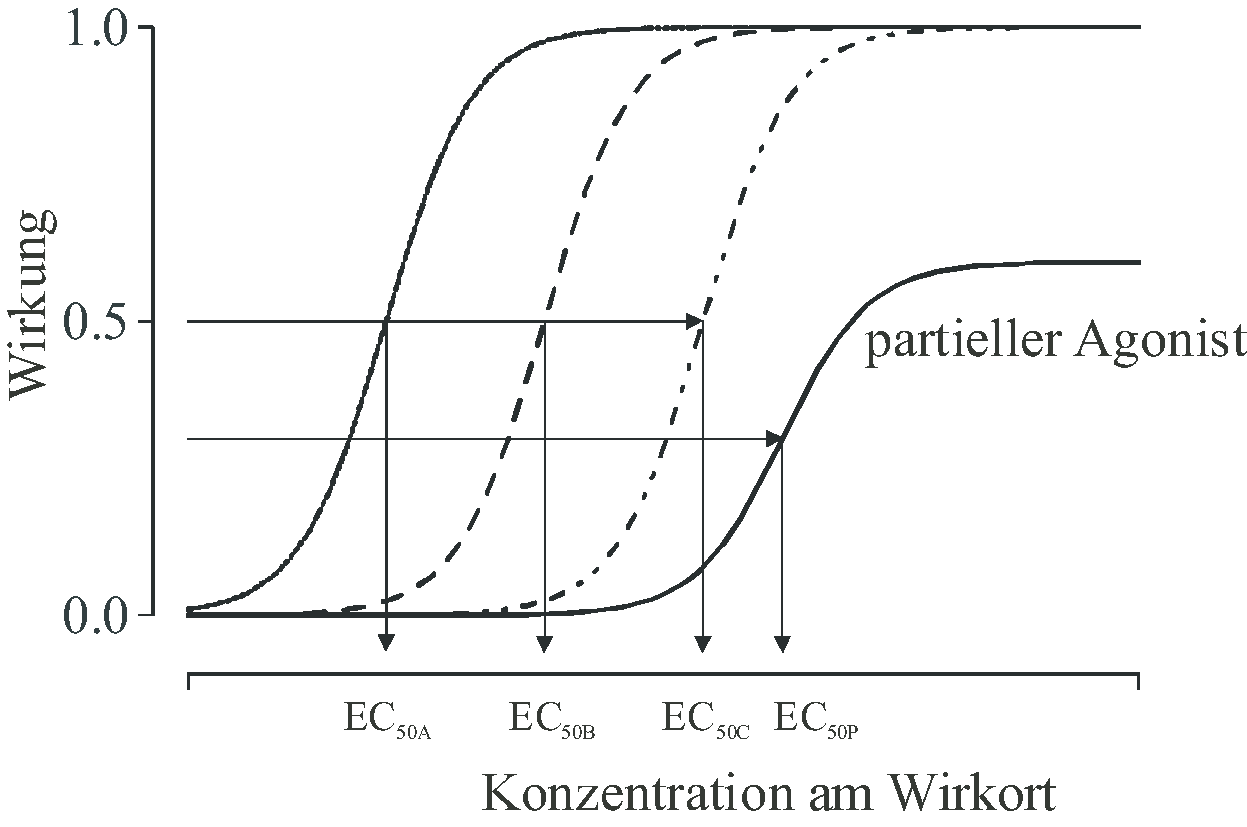
\includegraphics[clip=true,width=0.7\textwidth]{./pd2.pdf}
}

\note<1>{
Alle Begriffe erkl�ren.\\
Die Steigung ebenfalls einzeichnen.\\


Agonist und Antagonist haben eine ganz andere Wirkung am
Rezeptor. Agonist bindet sich und entfaltet eine Wirkung. Der
Antagonist bindet sich an den Receptor und bewirkt nichts. Falls
eine gewisse (partielle) Wirkung entfaltet wird spricht man von
einem partiellen Agonisten. }
\end{block}
}



